\documentclass[11pt]{article}

\usepackage{hyperref}
\usepackage{setspace}
\usepackage[pdftex]{graphicx}

\setlength{\oddsidemargin}{0.0in}
\setlength{\evensidemargin}{0.0in}
\setlength{\topmargin}{-0.25in}
\setlength{\headheight}{0in}
\setlength{\headsep}{0in}
\setlength{\textwidth}{6.5in}
\setlength{\textheight}{9.25in}
\setlength{\parindent}{0in}
\setlength{\parskip}{2mm}
\doublespacing

\begin{document}

\title{Bouncers: A Swing Application Utilizing JR Concurrency}
\author{Crystal Tse and Edmund Yan\\
  University of California, Davis, CA\\
  \texttt{cytse@ucdavis.edu, eyan@ucdavis.edu}}
\date{\today}
\maketitle

\begin{abstract}
The final assignment for ECS 140B: Programming Languages, Winter 2012 was to
apply the parallel programming constructs learned throughout the quarter to
a creative JR application with visuals from Java's Swing/AWT.  We created an
interactive video game called Bouncers, where multiple people (or one person)
click on soccer balls to prevent them from falling into a pit of fire.
\end{abstract}

\section{Introduction}

The inspiration for Bouncers came from a similar video game named Zurroball 
\cite{zurroball} on the popular website Neopets.  The basic game concepts
of preventing a ball from falling onto the ground were taken from here.  We 
expanded on this by adding multiple balls, levels, and a scoring system, and
also introduced a multiplayer aspect, so that players from different computers
 can work together towards the goal.  By using JR, we were able to easily 
parallelize the basic game functionality such as moving balls and testing 
for collisions.  Additionally, the multiplayer portion was very simple, as JR 
uses transparent communication between its virtual machines--meaning at the 
programmer level, \texttt{send} and \texttt{receive} statements from remote 
operations have the same syntax as if they were for an operation that existed 
on the same virtual machine.

\begin{figure}
	\begin{center}
		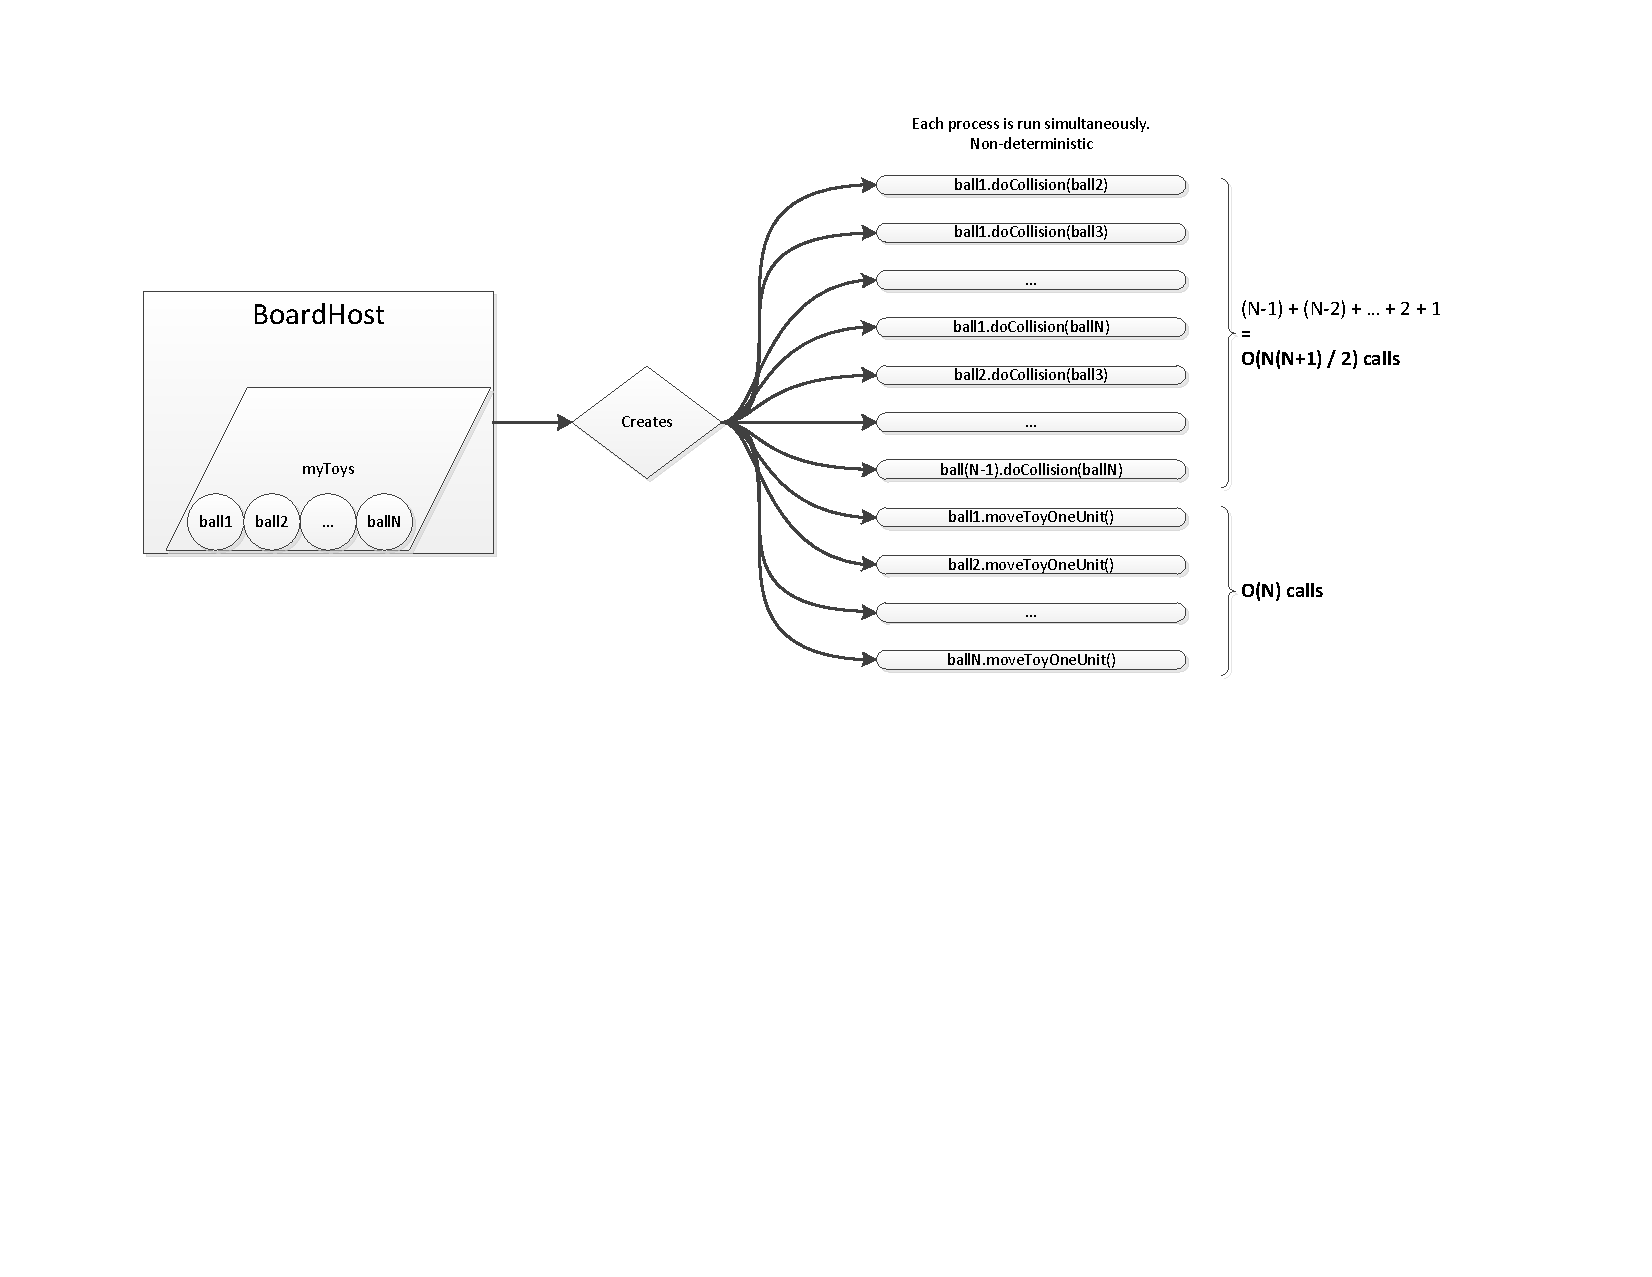
\includegraphics[viewport = 68 287 692 557, width=\textwidth]{fig1.pdf}
	\end{center}
	\caption{How BoardHost moves Ball objects}
	\label{fig1}
\end{figure}

\begin{figure}
	\begin{center}
		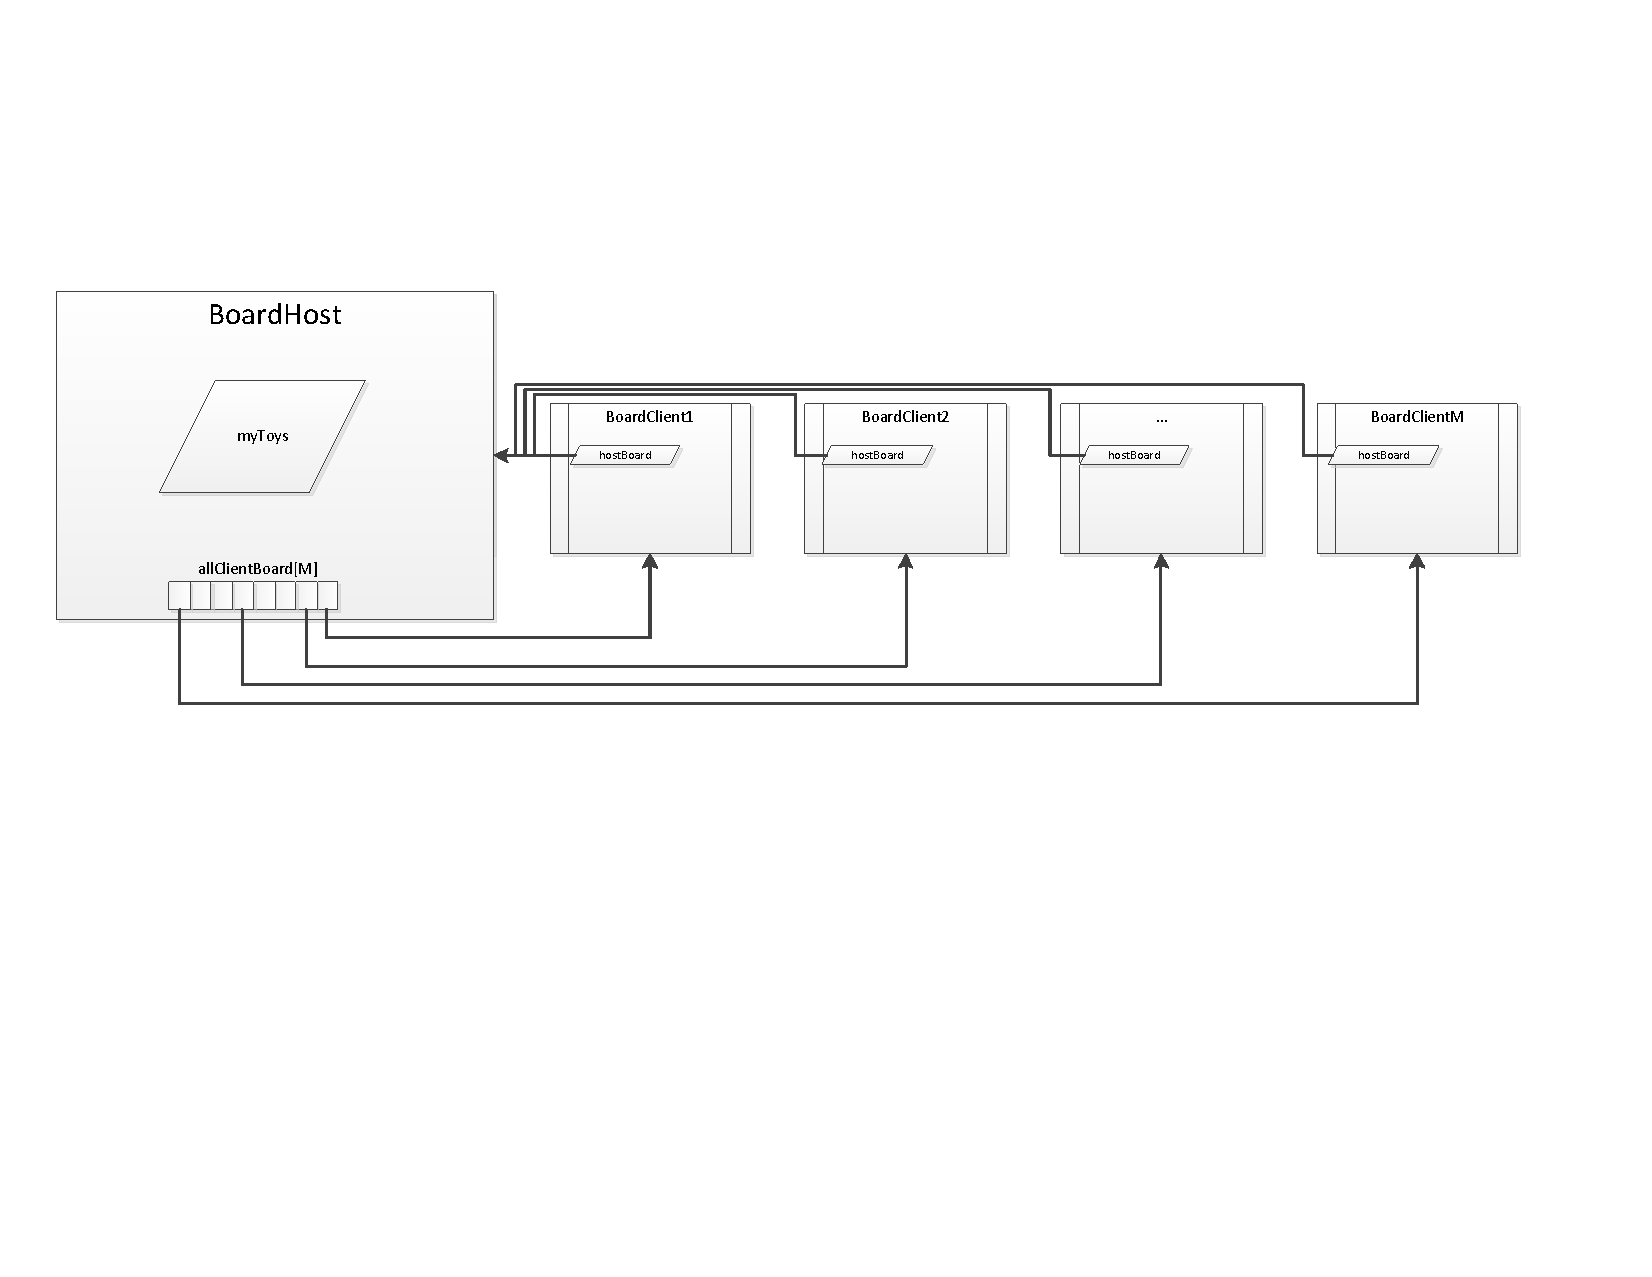
\includegraphics[viewport = 26 274 730 493, width=\textwidth]{fig2a.pdf}
	\end{center}
	\caption{How the multi-VMs are connected}
	\label{fig2a}
\end{figure}

\begin{figure}
	\begin{center}
		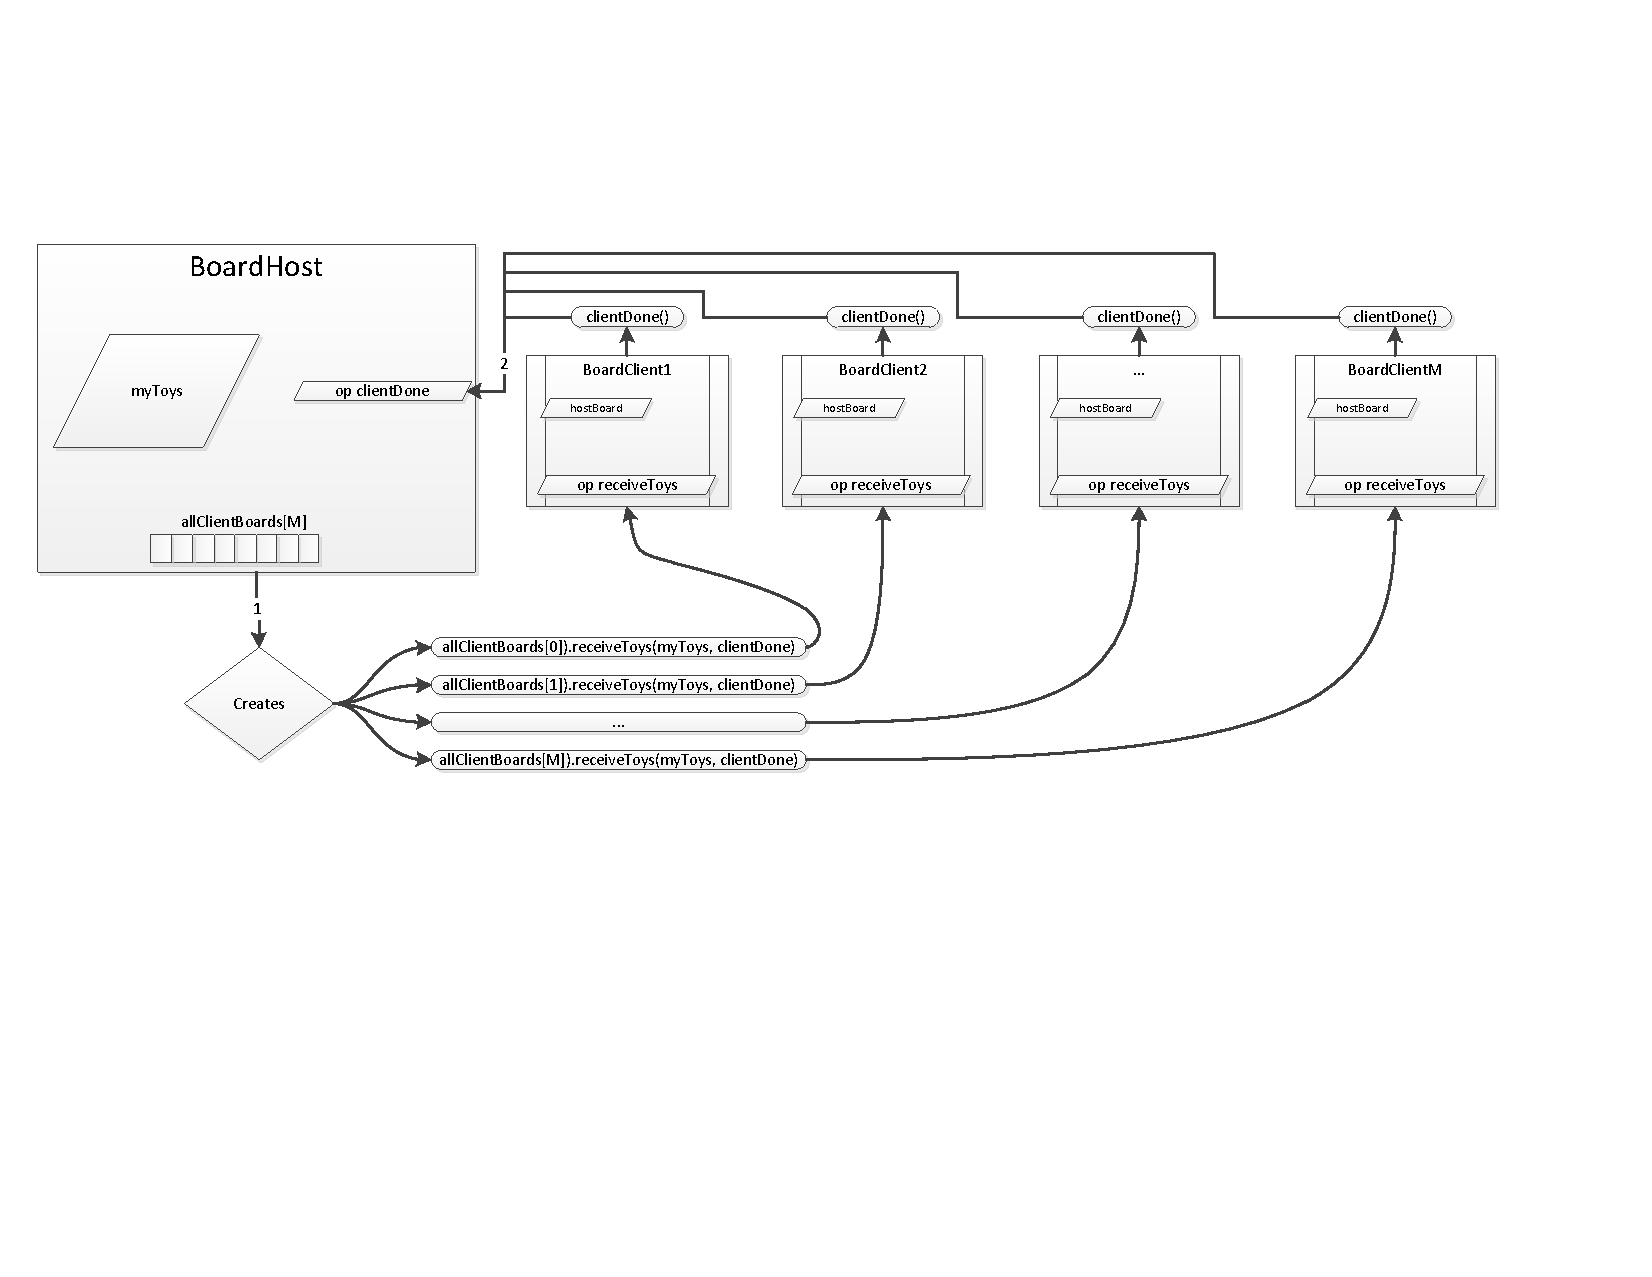
\includegraphics[viewport = 17 242 720 515, width=\textwidth]{fig2b.pdf}
	\end{center}
	\caption{How the multi-VMs communicate}
	\label{fig2b}
\end{figure}

\section{Project Design}
The design of Bouncers was based off of the game BnB \cite{JRBook}.  We used
BnB as a template for our first version of Bouncers, and slowly expanded it
from there.  Much of the class structure is kept the same, such as having a
Board class which manage the creation and movement of Ball objects.  There
is a SwingAppplication class that deal with creating and updating all of the 
Swing GUIs such as labels, buttons and text.
\\
When supporting multiplayer, the class structure of Bouncers changes 
dramatically from the typical structure shown in BnB.  In a world with 
multiple virtual machines, there is a single "host" virtual machine and many
"client" virtual machines.  The host in this case is a BoardHost object and
all of the clients are BoardClient objects.  Both of these classes are 
subclasses of the parent class Board.  This object oriented approach was
very helpful, as it provided a way to combine shared functionality between
a host's board and a client's board.


\section{Class Structure Overview}

\subsection{Main}
The Main class is where the program immediately begins after execution.  If 
there are no command line arguments, a single remote BoardHost object will be
created on \texttt{localhost} and an asynchronous \texttt{send} command to the 
object's goahead operation will occur.  If command line arguments are given, 
the first string will be used as the machine where the remote BoardHost object
will exist and any additional strings will have a remote BoardClient object 
created on them.  Each command line argument will be a machine name.  On that 
machine, there will be a new JR VM created with a Board object, Window Object,
and SwingApplication object.
 
\subsection{Window}
The Window class is used by both the host VM and client VM(s) to setup the GUIs
in JPanel and create the Board and SwingApplication objects.  The Window
constructor will also pass Board capabilities into the SwingApplication object 
so that it can communicate with the Board.

\subsection{SwingApplication}
The SwingApplication class is the main controller of the GUI aspects the 
player sees and interacts with on the Window.  Once createComponents is called
(from Window's constructor), a new Timer object is setup to trigger the 
ActionListener, taskPerformer, every tenth of a second.  The ActionListener 
uses the Board capabilities passed into the function as parameters to retrieve
the current game state ("Game Over" or "Loading"), current game points, and 
the current level.  Additionally, every 20 seconds (or \texttt{maxCounter} 
number of triggers), the ActionListener will tell the Board to drop two 
additional balls onto the field and increase the current level.

\subsection{Board}
The Board class is a base class that provides the fields and methods that all 
boards have in common.  Since all Boards look the same and have the same 
things, the constructor loads up the graphics and creates a list of toys 
(myToys).  Another thing Boards have in common is the paintComponent() method, 
which paints the background and all the toys.  Board also defines the 
operations that are essential for game play: newLevel(), plusPoints(), 
getPoints(), and startBall(). 
\\
The two classes that extend from Board are BoardHost and BoardClient.  In the 
case of a single-player game, only BoardHost is used; in the case of 
multi-player game, both are used.  On the surface, BoardHost does all 
computation for toy movement and sends the updated list of myToys to 
BoardClient, while BoardClient receives myToys and simply displays them in the 
aforementioned paintComponent() method.  This provides the desired effect of 
replicating the screen on all virtual machines.  More implementation details 
follow.

\subsubsection{BoardHost}
BoardHost extends the Board class.  The board code contains a startup process 
to handle board start up (receiving remote references for allclientBoards), 
waiting for allClientBoards to be initialized, and starting the boardManager.  
boardManager is an overridden operation that controls all ball movement and
collision, then repaints all balls to the screen.  An important thing to note
is that after calculating the next positions of all balls, boardManager sends
the list of myToys to allClientBoards, then waits to receive clientDone until
it can proceed.  
\\
Another overridden operation is mymouseclick, which is triggered whenever 
“this” board receives clicks, or when anyone in allclientBoards sends a click.
Each click “punches” the ball up, so this part determines ball movement and 
increases the game points.  If a ball has been clicked, mymouseclick sends a 
message to allClientBoards’ plusPoints operation, telling them to update their 
points.  Another important thing to note is that allClientBoards only has to 
update points, and nothing else, because BoardHost will take care of the rest.
\\
Other overridden operations are gameOver, which stops the game when one balls 
hits the bottom of the screen, and restartBoard, which starts up a new game 
and resets all game values.  Similarly to the previous operations, these also 
send messages to allClientBoards.  Also as before, allClientBoards need only 
minimal information—for gameOver, allClientBoards flips their gameStatus bit; 
for restartBoard, allClientBoards sets resets initial game values and sends a 
message to BoardHost.  
\\
Another important thing to note is that whenever BoardHost needs to iterate 
through myToys, it uses the Java synchronized statement to provide mutually 
exclusive access to the myToys collection.  This ensures that other processes 
do not change myToys while the iterator is going through the collection.  This 
is important because, for example, we don’t want to get a toy’s position and 
do collision detection based on that position, only to have that position be 
changed somewhere else.

\subsubsection{BoardClient}
BoardClient also extends the Board class.  This class is used if the game is 
being played on multiple virtual machines.  In its startup process, the 
receives a link to the hostBoard, sends a goahead to the hostBoard to notify 
it that we are created, then starts up boardManager().  Unlike hostBoard’s 
boardManager, this one merely has a loop that receives the list of myToys 
(sent from hostBoard), sends back the clientDone capability to notify 
hostBoard that we received myToys, then refreshes the screen to account for 
the updated toys.  Similarly, the mymouseclick() operation, which gets called 
when “this” board receives clicks, merely sends a message to boardHost’s 
mymouseclick operation, which handles the calculations.  The restartBoard 
operation is slightly different, because any Board can click “Start Game” to 
start a new game.  If the player on a BoardClient starts a game, restartBoard 
sends a message to boardHost’s  restartBoard operation, which takes care of 
notifying all the other BoardClients.  
\subsection{Toy}
Toy is the base class for clickable objects that appear on the screen, 
providing the mutators and accessors for the class variables. In the
current version of Bouncers, only the Ball class is derived from Toy.

\subsection{Ball}
The Ball class is a child of the Toy class.  We take advantage of Java's 
static class variables by declaring \texttt{image\_scaled} as static.  In 
Bouncers, each Ball object draws an image of a soccer ball onto the screen 
instead of a solid-color circle.  Rather than having each Ball object read the
file from disk, the Image variable is stored once in memory and only read from
disc the first time a Ball object is created.

\subsubsection{Physics}
All of the physics and movement mechanics of the game are defined within the 
operations of the Ball class.  The physics and algorithms for 2D ball 
collisions have been implemented many times before, and we drew a lot of our
inspiration from the help of online websites
\cite{ballcollisionsA}\cite{Chuan}.  All of these operations are used by the
BoardHost class to simulate ball movements and collisions.
\subsubsection{KeyInput / MouseInput}
The MouseInput class takes a capability (mouseClick) for an operation in its 
board to which the (x, y) coordinates are to be sent.  We use mousePressed 
because it’s faster than mouseClicked, because mouseClicked coalesces the 
clicks together.  The KeyInput class doesn’t need a capability, because we 
only use the keyboard to handle exiting the game.


\section{Improvements}
Pete Doctor, the director of Pixar's UP, once said that "Pixar films don't get 
finished, they just get released".  While we are extremely satisfied with the 
current state of Bouncers, we would have loved the opportunity to spend more 
time with the game and improve it.  Here are some things we would have loved 
to implement if we had more time:

\subsection{Game Mechanics}
There are lots of cool things that we could add to make the "game" aspect more 
fun.  For one, the Toy class was created to allow us to easily create 
different types of Toys.  Currently, there is only a single Ball class, but we
would have loved to expand this. Some interesting ideas tossed around were:
\begin{itemize}
\item "Bombs" that look similar to Balls but would end the game immediately 
			if a player tried to punch it.
\item Balls with different sizes and speed.
\item Power-Ups that when punched, altered the game state (adding more points, 
			slowing down the game, etc.).
\end{itemize}

\subsection{Multi\-VM Speed Optimizations}
The current host and client VM structure made the program very easy
to convert from a single player game to a multi-player game (the main reason
we chose this path).  However, the performance of the game dips dramatically 
with this method.  The reason is that every time step, the host must send to
each client a full copy of the \texttt{myToys} list.  The client receives the
list and simply does a \texttt{repaint()} method call.  Here, the processing 
power of the client is not used at all.  A possible solution  is to have the 
host send \texttt{myToys} every T time steps to each client.  The times where 
no data is sent, the clients will simulate their own physics.  This would cut
down the number of synchronization steps by a linear factor of T.

As the number of balls gets larger, the time to compute one time step for all
of the balls becomes very long and the slowdown is noticable to the user.  An
obvious fix would be to divide the work (collisions and movement) into chunks
so that other PCs are able to compute and simply send back the result to the 
host.

\section{Conclusion}
Bouncers was an extremely fun and rewarding program to write.  We learned
a lot about being able to read and understand every part of someone else's code
(BnB).  This is an important lesson, as in the real world, you often face the
task of maintaining code that was not originally yours or having to integrate
foreign code to your own.  We learned about Swing and had a real hands on 
approach to creating a large application using JR.


\begin{thebibliography}{9}
	% IEEE Style
	\bibitem{JRBook}
	  A. Keen and R. Olsson,  % Author
	  \emph{The JR Programming Language:  Concurrent Programming in an 
	  			Extended Java}.	% Title
		Norwell, MA:	% City of Publisher
		Kluwer Academic Publishers,	% Publisher
		2004.	% Year of Publication
	\bibitem{ballcollisionsA}
		BlueThen,
		[Online]
		Available:
		\url{http://bluethen.com/wordpress/index.php/processing-app/do-you-like-balls/}
	\bibitem{Chuan}
		C. Chuan,
	  \emph{Java Game Programming: Introduction - The World Of Bouncing Balls}.	% Title
		[Online]
		Available:
		\url{http://www3.ntu.edu.sg/home/ehchua/programming/java/J8a_GameIntro-BouncingBalls.html}
	\bibitem{zurroball}
		Neopets Inc.,
		[Online]
		Available:
		\url{http://www.neopets.com/games/zurroball.phtml}
\end{thebibliography}



\end{document}
